\section{Wallclock sampling}\label{app:moses-wallclock}

Figure~\ref{fig:moses-vun-wallclock} reports the MOSES wallclock view of V.U.N.\ (WiP).

\begin{figure}[t]
\centering
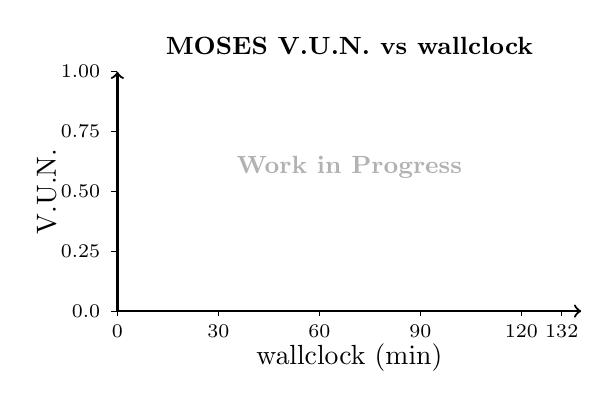
\begin{tikzpicture}[scale=0.95]
  \draw[->, thick] (0,0) -- (6.2,0) node[midway, below=8pt] {wallclock (min)};
  \draw[->, thick] (0,0) -- (0,3.2);
  \node[rotate=90] at (-0.95,1.6) {V.U.N.};

  % Title
  \node[font=\small\bfseries] at (3.1,3.55) {MOSES V.U.N. vs wallclock};

  % Axes ticks
  \foreach \x/\lab in {0/0,1.35/30,2.70/60,4.05/90,5.40/120,5.94/132} {
    \draw (\x,0) -- (\x,-0.06);
    \node[below, font=\scriptsize] at (\x,-0.06) {\lab};
  }
  \foreach \y/\lab in {0/0.0,0.8/0.25,1.6/0.50,2.4/0.75,3.2/1.00} {
    \draw (0,\y) -- (-0.08,\y);
    \node[left, font=\scriptsize] at (-0.1,\y) {\lab};
  }

  % Placeholder text
  \node[gray!60, font=\small\bfseries] at (3.1,1.92) {Work in Progress};
\end{tikzpicture}
\caption{\footnotesize Fraction of valid, unique, and novel (V.U.N.) versus wallclock on MOSES, on a single H100 with 1k samples and batch size 128. \textcolor{red}{[WiP]}}
\label{fig:moses-vun-wallclock}
\end{figure}
